% !TEX root = catron-dissertation.tex
\epstopdfsetup{outdir=./images/06_single_sensor_filtering/}

\chapter{Single Sensor Filtering Techniques}

\textcolor{red}{Show some dispersions of POD modes and discuss whether or not POD filtering maybe a viable option.}

A filter is a function, $G(\mathbf{\omega})$, that describes the gain a signal will experience in frequency space.
In the simplest case, the filtered signal is the inverse Fourier transform of the gain multiplied by the Fourier transform of the signal.
Additionally, a windowing function, $W(\mathbf{x})$, can be used to help suppress finite sampling effects,
\begin{equation}
 f_F(\mathbf{x}) = \real\left(\frac{\ifftn[G(\mathbf{\omega})\cdot\fftn\{f(\mathbf{x})\cdot W(\mathbf{x})\}]}{W(\mathbf{x})}\right) \textrm{,}
 \label{eqn:06_filter_function}
\end{equation}
where $f$ is the signal function and $f_F$ is the filtered signal.
Depending on the windowing function some data could be destroyed during this process if there is a zero present due to the possibility of dividing by zero.

A basic MATLAB code for applying a filter to a wavefront using a separate function for both generating and applying the gain function which is presented in Listing \ref{code:sc_basic_wavefront_filters}.
This code generates a windowing function as described by Equations \ref{eqn:04_hann_window}, \ref{eqn:04_window_sep}, and \ref{eqn:04_window_space_arb}.
The temporal windowing function was generated with an additional two terms such that the end points which are equal to zero could be removed to prevent the first and last frames from being destroyed.
Likewise, the spatial window used the arbitrary aperture function which ensures that all of the points inside of the aperture are non-zero.
In some cases, a windowing function was not used due to filtered wavefront having a far greater magnitude in some places despite the precautions used.
The filter presented in this code sample is a second order temporal high-pass filter with a cut-off frequency of 2000 Hz.
The function \lstinline{WFfilter} takes input based on a normalized cut-point in reference to the sample rate.

\section{Temporal Filter Methods}
The methods presented in this section are based on Butterworth filters \cite{Butterworth-1930-DvDrjKha} but could easily be extended to other types of filters.
The basic gain function,
\begin{equation}
 G(f) = \frac{1}{\sqrt{1+\left(\frac{f}{f_c}\right)^{\pm2n}}} \textrm{,}
 \label{eqn:06_butterworth}
\end{equation}
where $f_c$ is the cut-off frequency, $n$ is the filter order (number of filters in a series), and $\pm$ represents either a low-pass ($+$) or high-pass ($-$) filter.
In this particular formulation, only the magnitude is attenuated, circuit based Butterworth filters or their digital copies will have some variable phase attenuation as well.
Additionally, a band-pass filter can be constructed by placing a low-pass in series with a high-pass filter and a band-stop by placing the two types in parallel.

As a large portion of the wavefront contamination is at low frequencies, a high-pass filter is the most useful in temporal space for removing unwanted contamination, as shown in Figure \ref{fig:06_filter_temporal}.
\begin{figure}
 \centering
 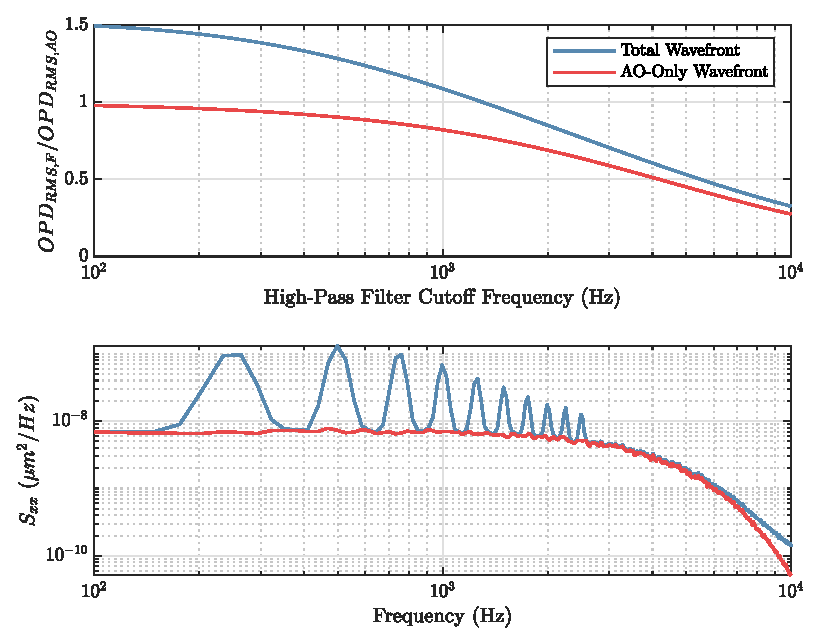
\includegraphics{../matlab/06_single_sensor_filtering/filter_temporal.eps}
 \caption{OPD time-averaged spatial-RMS of high-pass temporal filters relative to the aero-optical only unfiltered wavefront.}
 \label{fig:06_filter_temporal}
\end{figure}
This figure shows the time-averaged spatial-RMS of both the total and aero-optical only wavefronts with various cut-off high-pass filters relative to that of the aero-optical only wavefront unfiltered.
The total wavefront ratio crosses unity around 1200 Hz, which is about halfway between the second and third harmonic of the blade-passing frequency in this simulated wavefront.
While approximately 75\% of the aero-optical signal remains at this cut-off frequency, that difference is made up by the remaining contamination.
This can provide a computationally cheap way estimating the aero-optical portion of the wavefront for calculations that rely on the spatial-RMS of a wavefront.
While it is easy to determine a cut-off frequency for this synthetic wavefront, a measured wavefront will likely take some knowledge or expectation of the contamination that is present in the measurement.

% \ref{tab:test}
% \begin{table}
% \centering
% \caption{Test Table}
% \input{../matlab/04_basic_filtering/filter_temporal.txt}
% \label{tab:test}
% \end{table}

An example of band-pass and band-stop filtering is shown if Figure \ref{fig:06_filter_temporal_bandpass}.
\begin{figure}
 \centering
 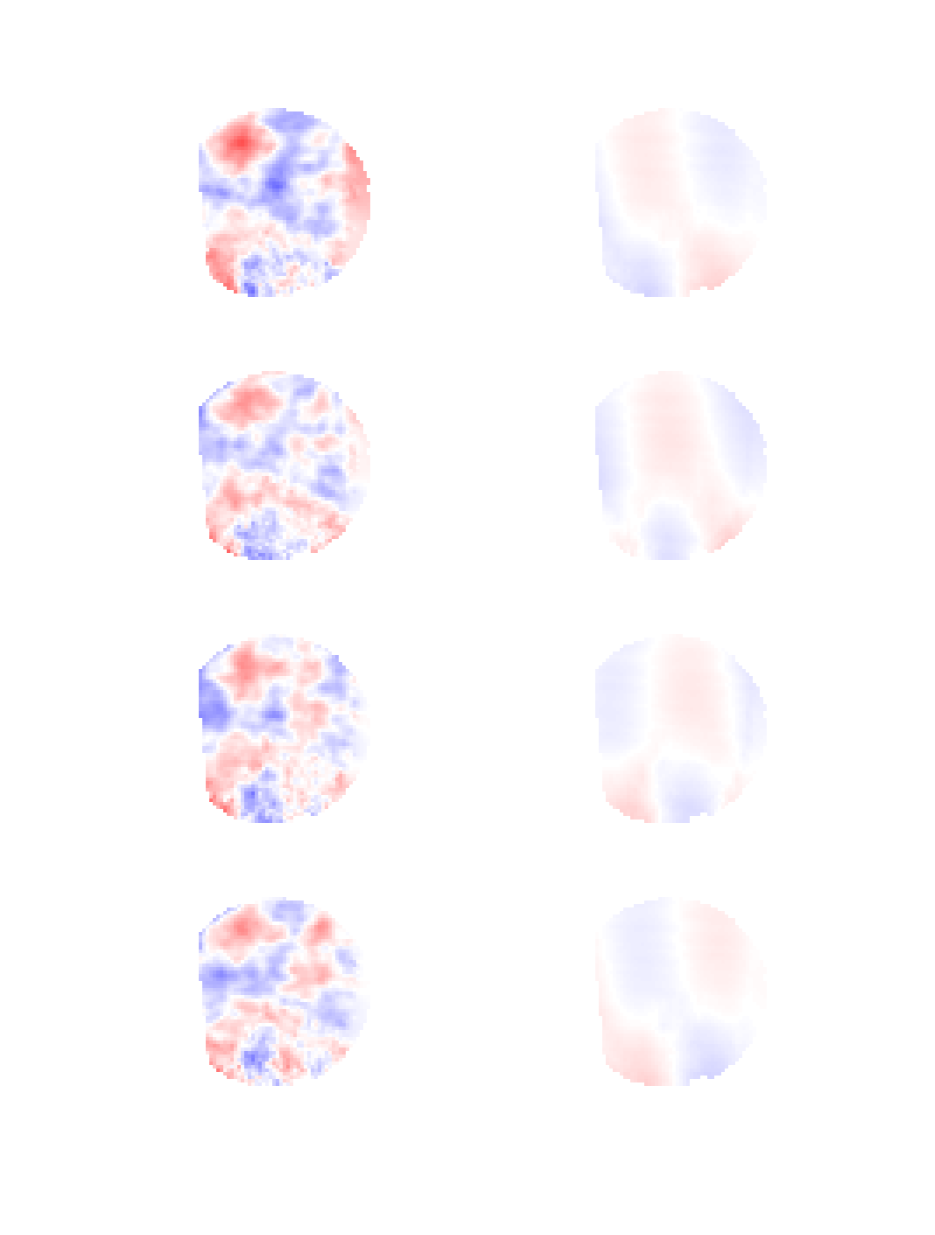
\includegraphics{../matlab/06_single_sensor_filtering/filter_temporal_bandpass.eps}
 \caption{Measured wavefronts filtered at the blade-passing frequency (532$\pm$10 Hz).  The left column is band-stop filtered while the right is band-pass filtered.}
 \label{fig:06_filter_temporal_bandpass}
\end{figure}
The figure shows measured data that is band-stop filtered in the left column and band-pass filtered in the right column in several different frames.
The flow is from right-to-left and the band-pass filtered wavefront clearly shows upstream-moving optical disturbances associated with acoustic duct modes traveling upstream from the fan.
The band-stop shows a much slower moving optical disturbance that is in general moving in the direction of the flow, but it still possess the optical disturbances of the blade-pass frequency harmonics.

One thing of note, MATLAB's builtin filter functions only work in one-dimension of frequency space and are unable to determine the direction that a signal is traveling.
They also only apply the filter to the positive frequencies and zero-out the negative ones which both reduces the signal by two and also switches all disturbances to moving in the same direction.
So even for a filter that operates in one-dimension, it is best to apply the filter over both positive and negative frequencies to the n-dimensional Fourier transform in order to preserve the direction of travel of a signal.
This additionally allows several filters to be applied in series with one another without having to perform a Fourier and inverse Fourier transform for each successive filter.
\textcolor{red}{I should maybe show this matlab filter issue in an appendix.}

Some additional uses of temporal filters would be in sizing and/or designing an adaptive optics system.
A low-pass filter with a cut-off at the bandwidth of either a fast-steering or deformable mirror would help determine the signal that a system would need to reject.
A control system may need to have the bandwidth reduced in order to keep a mirror's travel within limits.
While a high-pass filter would inform designers of the remaining optical aberrations that cannot be corrected.




\section{Upstream/Downstream Moving}
For the filtering of upstream and downstream moving optical disturbances a logistic function was chosen,
\begin{equation}
 f(x) = \frac{1}{1+\exp\{-kx\}} \textrm{.}
 \label{eqn:06_logistic}
\end{equation}
This function needs to be expanded into two-dimensions ($x$ and $t$) with the filter ideally returning a value of one in both the first and third quadrants and zero otherwise for a filter outputs disturbances moving in the direction of flow.
To accomplish this the logistic curve in each dimension is scaled and offset to output values between negative one and positive one,
\begin{equation}
 G_t(f) = \frac{2}{1+\exp\{-k_tf\}}-1
 \label{eqn:06_logistic_time}
\end{equation}
and
\begin{equation}
 G_x(\xi_x) = \frac{2}{1+\exp\{\pm k_x\xi_x\}}-1 \textrm{,}
 \label{eqn:06_logistic_space}
\end{equation}
where $\pm$ determines whether the filter is obtaining upstream traveling disturbances ($+$) or downstream traveling ($-$).
These two gain functions are then multiplied together and scaled to output values between zero and one,
\begin{equation}
 G(\xi_x,f) = \frac{(G_t\cdot G_x)+1}{2} \textrm{.}
 \label{eqn:06_up_down_filter}
\end{equation}
As the values of $k_x$ and $k_t$ go to infinity an ideal case is obtained.
Downstream traveling disturbances have a gain of one in the first and third quadrants, zero in the second and forth quadrants, and a value of $1/2$ when either frequency is zero.

The dispersion analysis using an ideal downstream moving filter on the synthetic wavefront is shown in Figure \ref{fig:06_filter_downstream} along side the dispersion of the unfiltered wavefront.
\begin{figure}
 \centering
 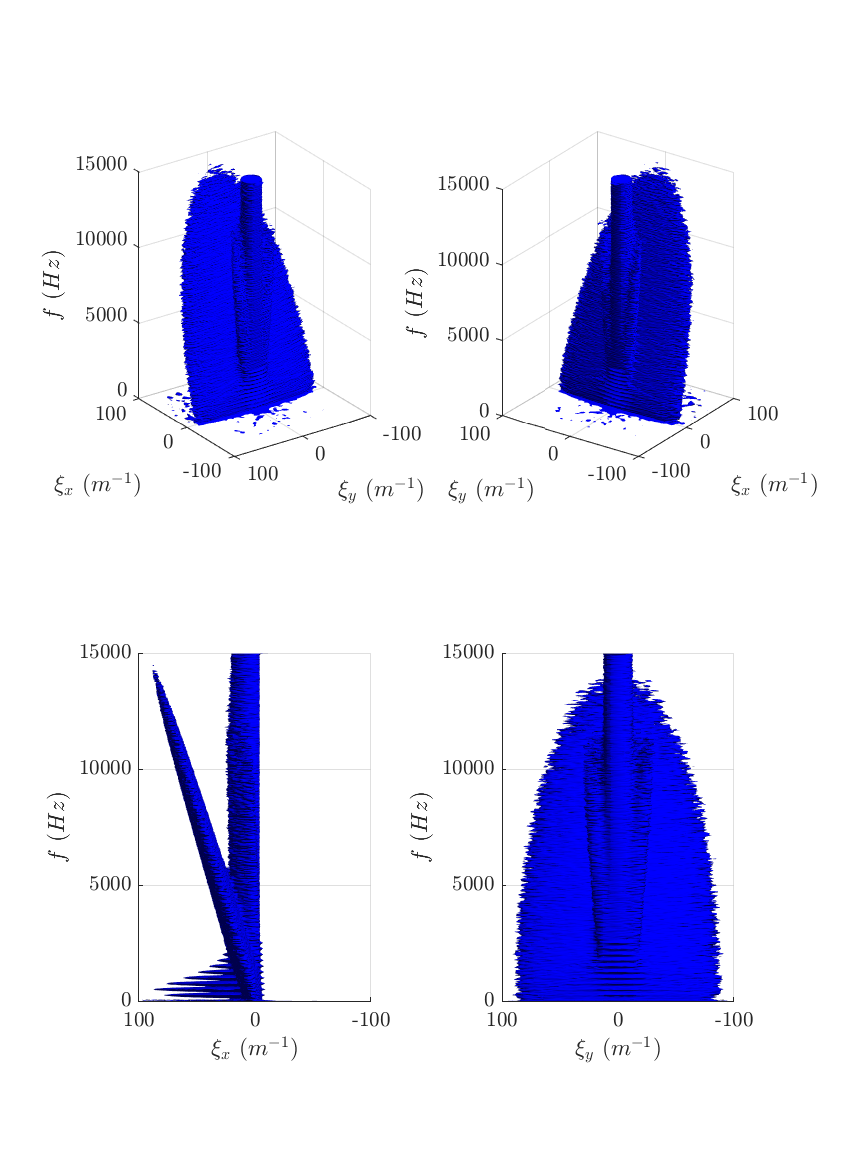
\includegraphics{../matlab/06_single_sensor_filtering/filter_downstream.eps}
 \caption{Dispersion isosurface of the synthetic wavefront with a downstream filter in place.}
 \label{fig:06_filter_downstream}
\end{figure}
All of the upstream traveling disturbances are removed and the disturbances at $\xi_x=0$ m$^{-1}$ are significantly reduced.
Some of the stationary modes remain while only the acoustic and vibration signals that are propagating in the direction of flow remain.
The aero-optical signal is clipped slightly at $\xi_x=0$ due to the spatial width of the signal.
The ratio of the time-averaged spatial-RMS of the filtered signal when compared to the aero-optic only signal was 1.24 while the unfiltered ratio was 1.53.
When the filter was applied to only the aero-optic signal the ratio was 0.96.
This filter method will retain any disturbance that is traveling in the direction of flow.
Even with an ideal filter there is some slight attenuation of the aero-optical signal due to signal having some spectral width that crosses into upstream-moving portion of the dispersion plot.


\section{Velocity Filtering}
The dispersion plot shows flow structures that are traveling at a given speed as having a constant slope.
A plane in the dispersion plot can be used to measure a flow structure's velocity in both $x$ and $y$-directions.
The distance from any given point in the dispersion plot to a plane described by the velocities $v_x$ and $v_y$ can be computed by
\begin{equation}
 d = \frac{|v_x\xi_x+v_y\xi_y-f|}{\sqrt{v_x^2+v_y^2+1}} \textrm{.}
 \label{eqn:06_dist_point_2_plane}
\end{equation}
A low-pass or high-pass filter can then be used to retain only disturbances that are traveling at that velocity, or to exclude those disturbances respectively.

A low-pass velocity-filter of the synthetic wavefront is shown in Figure \ref{fig:06_filter_velocity}.
\begin{figure}
 \centering
 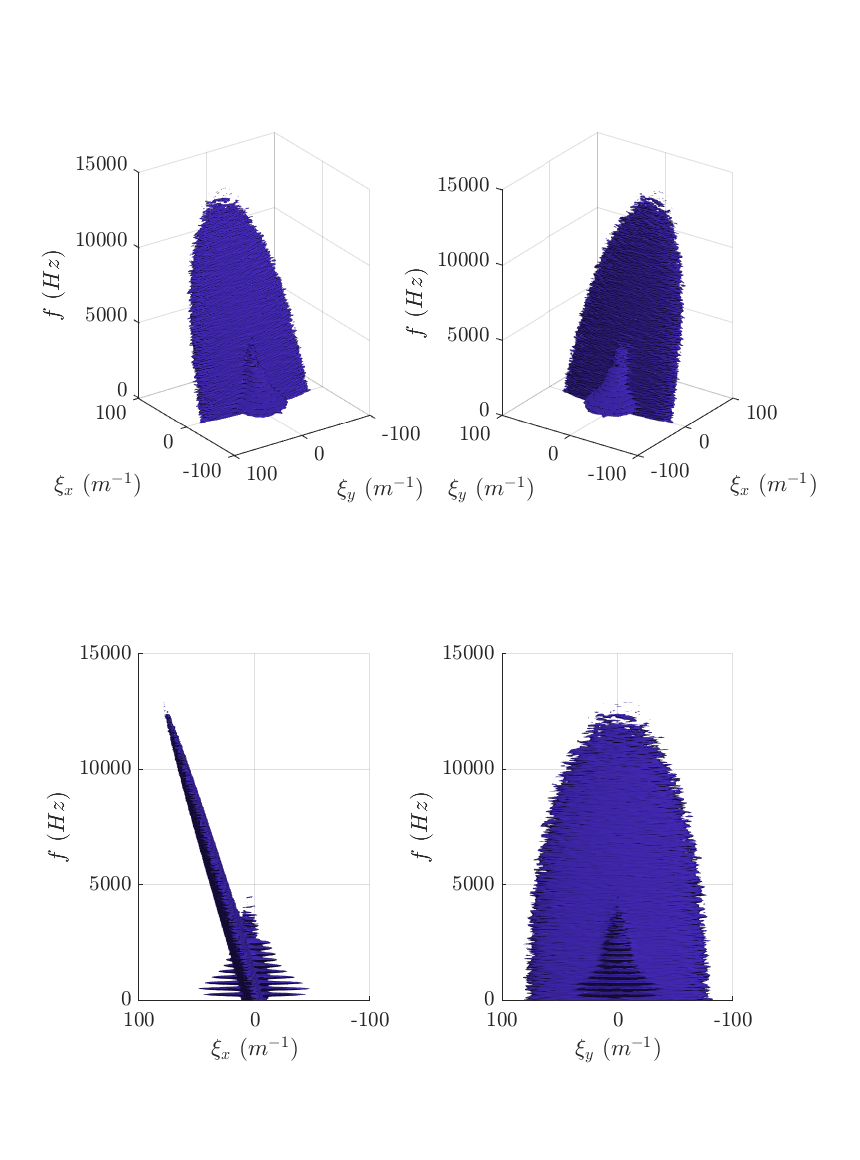
\includegraphics{../matlab/06_single_sensor_filtering/filter_velocity.eps}
 \caption{Dispersion isosurface of the synthetic wavefront with a low-pass velocity-filter in place.}
 \label{fig:06_filter_velocity}
\end{figure}
The filtered dispersion plot shows primarily only the aero-optic signal remains with some additional low-frequency content from the blade-passing frequency and harmonic disturbances as well as some stationary and acoustic disturbances.
The ratio of the time-averaged spatial-RMS relative to that of the aero-optical only signal went from 1.53 in the unfiltered case to 1.01 in the filtered case.
This method can provide a very effective way in quickly estimating the clean spatial-RMS of a contaminated wavefront.

Another use of the synthetic wavefront is measuring the speed of a broadband disturbance such as the aero-optical signal of a boundary layer.
This is done by finding the velocity that maximizes the output spatial-RMS of the velocity filter, see Figure \ref{fig:06_filter_velocity_measure}.
\begin{figure}
 \centering
 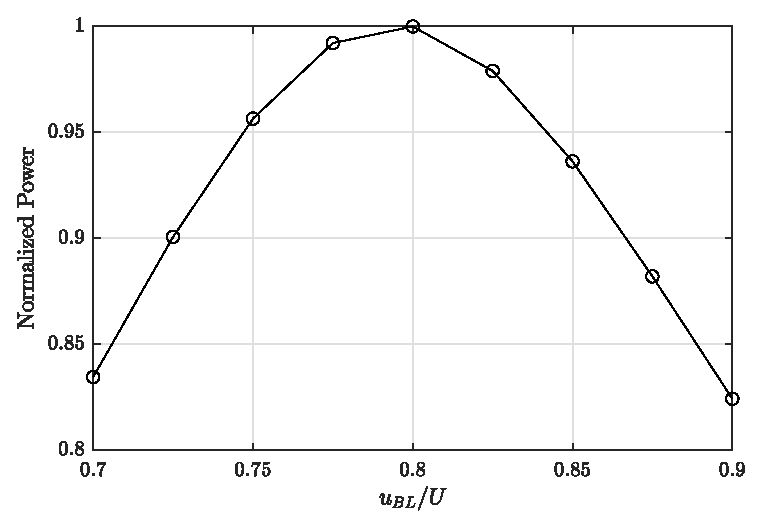
\includegraphics{../matlab/06_single_sensor_filtering/filter_velocity_measure.eps}
 \caption{Velocity low-pass filter used to determine the mean disturbance velocity.  The maximum value corresponds with the actual value used in the creation of the synthetic wavefront.}
 \label{fig:06_filter_velocity_measure}
\end{figure}
In this case boundary layer speed was determined to be 163 m/s which corresponds to the design velocity of the synthetic signal of $0.8U$.
If the velocity range used is to large, a false result can be obtained due to the inclusion of disturbance structures not related to the aero-optical signal.
For signals that have a mean-velocity component that is not aligned with an axis both velocity components can be varied as shown in Figure \ref{fig:06_filter_velocity_real}.
\begin{figure}
 \centering
 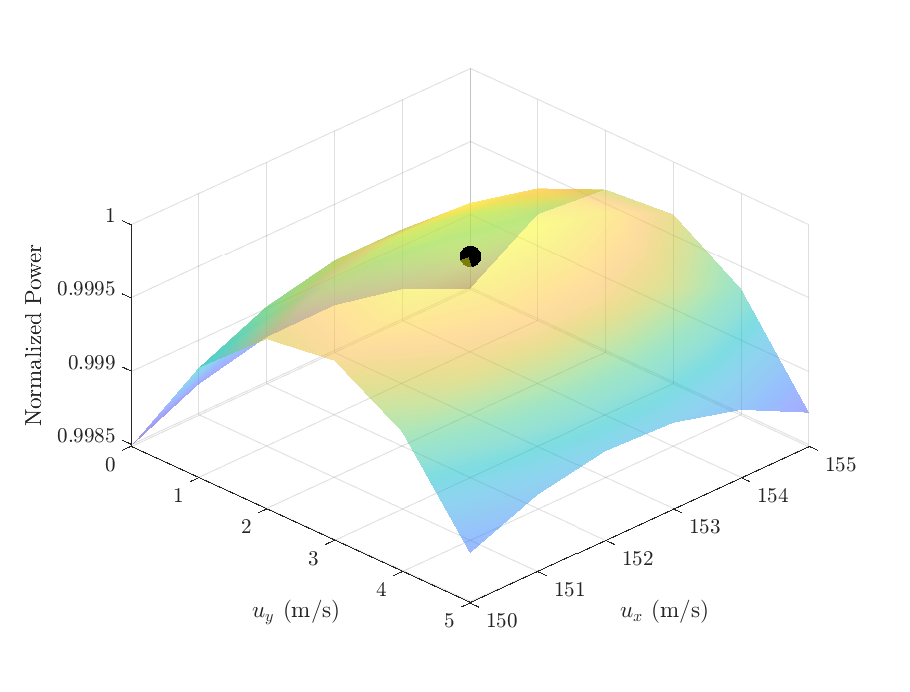
\includegraphics{../matlab/06_single_sensor_filtering/filter_velocity_real.eps}
 \caption{Velocity low-pass filter used to determine the mean disturbance velocity of measured data presented in Figure \ref{fig:06_dispersion_real}.  The velocity in the x-direction was measured to be 207 m/s and -17 m/s in the y-direction.}
 \label{fig:06_filter_velocity_real}
\end{figure}
In this case a variable low-pass velocity filter was employed with a high-pass spatial filter operating in the radial direction.
This helped eliminate some of the low-frequency stationary disturbances as well as some of the disturbances related to the blade-passing frequency.
The velocity was measured using the optical disturbances in the dispersion plot to be approximately 207 m/s in the x-direction and -17 m/s in the y-direction.

\section{Basic Filter Summary}
Three different basic wavefront filters were shown and discussed in this chapter.
The temporal filter is most useful when separating an optical wavefront into frequency bands.
Adaptive optics system performance can be evaluated by using both high-pass and low-pass temporal filters.
High-pass filters can be used to determine a systems performance that cannot be corrected while low-pass filters can be used to sizing the travel of active optical components.
Band-pass filters are helpful in analyzing a wavefront over a narrow-band to examine the optical aberrations at specific frequencies that significantly contribute to the overall optical disturbance.

Filters that separate upstream and downstream-moving disturbances are useful as most of the optical contamination comes from acoustic signals that are traveling upstream form a wind-tunnel fan.
These filters would also be useful for separating out an aero-optical signal that has a broad range of velocities that can occur in a span wise measurement of a boundary layer.
\textcolor{red}{Use some of sontag's data and site his dissertation.}

The velocity filter is the most useful for isolating the aero-optical portion of a wavefront measurement given the aero-optical signal has a fairly narrow and constant velocity range.
By using this filter to maximize the power over a range of velocities it can be used to measure the speed in both x and y-directions of an optical disturbance.
